% CVPR 2022 Paper Template
% based on the CVPR template provided by Ming-Ming Cheng (https://github.com/MCG-NKU/CVPR_Template)
% modified and extended by Stefan Roth (stefan.roth@NOSPAMtu-darmstadt.de)

\documentclass[10pt,twocolumn,letterpaper]{article}

%%%%%%%%% PAPER TYPE  - PLEASE UPDATE FOR FINAL VERSION
\usepackage[review]{cvpr}      % To produce the REVIEW version
%\usepackage{cvpr}              % To produce the CAMERA-READY version
%\usepackage[pagenumbers]{cvpr} % To force page numbers, e.g. for an arXiv version

% Include other packages here, before hyperref.
\usepackage{graphicx}
\usepackage{amsmath}
\usepackage{amssymb}
\usepackage{booktabs}
\usepackage{subcaption}  % Changed from subfigure to subcaption


% It is strongly recommended to use hyperref, especially for the review version.
% hyperref with option pagebackref eases the reviewers' job.
% Please disable hyperref *only* if you encounter grave issues, e.g. with the
% file validation for the camera-ready version.
%
% If you comment hyperref and then uncomment it, you should delete
% ReviewTempalte.aux before re-running LaTeX.
% (Or just hit 'q' on the first LaTeX run, let it finish, and you
%  should be clear).
\usepackage[pagebackref,breaklinks,colorlinks]{hyperref}


% Support for easy cross-referencing
\usepackage[capitalize]{cleveref}
\crefname{section}{Sec.}{Secs.}
\Crefname{section}{Section}{Sections}
\Crefname{table}{Table}{Tables}
\crefname{table}{Tab.}{Tabs.}


%%%%%%%%% PAPER ID  - PLEASE UPDATE
\def\cvprPaperID{*****} % *** Enter the CVPR Paper ID here
\def\confName{CVPR}
\def\confYear{2025}


\begin{document}

%%%%%%%%% TITLE - PLEASE UPDATE
\title{SoccerVision: Player Detection and Team Classification using Computer Vision Techniques}

\author{Abel Dagne\\
Department of Computer Science\\
Stanford University\\
{\tt\small abeldag@stanford.edu}
\and
Laszlo Bollyky\\
Department of Computer Science\\
Stanford University\\
{\tt\small lbollyky@stanford.edu}
% For a paper whose authors are all at the same institution,
% omit the following lines up until the closing ``}''.
% Additional authors and addresses can be added with ``\and'',
% just like the second author.
% To save space, use either the email address or home page, not both
}
\maketitle

%%%%%%%%% ABSTRACT
\begin{abstract}
   This paper presents SoccerVision, a computer vision system for detecting soccer players and classifying their team affiliations in match imagery. Instead of relying on complex deep learning models, we implement classical computer vision techniques including Canny edge detection, and custom k-means clustering for color-based team classification. Our approach first identifies player regions using edge detection and field segmentation, then classifies players into teams by analyzing jersey colors in HSV color space. The system demonstrates that effective player detection and team classification can be achieved with fundamental computer vision algorithms, without requiring external libraries or pre-trained models. Experimental results show the system can successfully detect players and classify them into appropriate teams across various soccer match scenarios.
\end{abstract}

%%%%%%%%% BODY TEXT
\section{Introduction}
\label{sec:intro}

Soccer (football) analytics has become an essential aspect of modern sports, with teams and broadcasters seeking automated ways to extract player information from match footage. While many commercial systems employ sophisticated deep learning approaches requiring extensive training data and computational resources, there remains value in exploring what can be achieved with fundamental computer vision techniques.

This project, SoccerVision, addresses the challenge of detecting soccer players on the field and classifying them into their respective teams using only classical computer vision algorithms. The system demonstrates how a combination of edge detection, color space manipulation, and clustering can produce effective results without relying on neural networks or external machine learning libraries.

The primary challenges in this domain include:
\begin{itemize}
    \item Distinguishing players from the field and background elements
    \item Handling variable lighting conditions across different stadiums
    \item Differentiating between teams based solely on jersey colors
    \item Managing occlusions when players overlap
    \item Processing images with sufficient speed for potential real-time applications
\end{itemize}

By addressing these challenges with classical computer vision approaches, this work serves as both a practical system and an easy accessible resource for collegite teams to analyze soccer matches.

\section{Related Work}
\label{sec:related}

The detection and tracking of sports players has been an active research area for decades. Early approaches relied primarily on background subtraction techniques, assuming a relatively static background (the field) against which players could be detected. These methods often struggled with changing lighting conditions and camera movements.

With the rise of deep learning, many recent approaches have shifted to using convolutional neural networks for player detection. These methods typically employ object detection frameworks such as Faster R-CNN, YOLO, or SSD to identify players in video frames with high accuracy. While effective, these approaches require substantial training data and computational resources.

For team classification, color-based methods remain common even in modern systems. Previous work has shown success using color histograms in HSV space to differentiate teams, while more recent approaches have employed clustering techniques on color features extracted from player regions. Other work has used machine learning models to identify teams based on features extracted from player regions \cite{SoccerCV2013}.

Our approach differs from recent work by intentionally avoiding deep learning methods, instead focusing on demonstrating what can be achieved with classical computer vision algorithms. This makes our system more accessible for educational purposes and deployable in environments with limited computational resources. Unlike some prior work that relies on sophisticated tracking algorithms across video frames, our system operates on individual images, making it applicable to both video and still image analysis.

\section{Methodology}
\label{sec:method}

Our approach consists of two main components: player detection and team classification. Each component utilizes classical computer vision techniques implemented without relying on external machine learning libraries.

\subsection{Player Detection}

The player detection pipeline employs a series of image processing steps to identify player regions within a soccer match image:

\begin{enumerate}
    \item \textbf{Grayscale Conversion:} The input RGB image is converted to grayscale to simplify subsequent processing.
    
    \item \textbf{Gaussian Blur:} A Gaussian blur with a 5×5 kernel is applied to reduce noise while preserving structural information necessary for edge detection.
    
    \item \textbf{Gradient Calculation:} Image gradients are computed using Sobel operators in both horizontal and vertical directions to identify regions with intensity changes.
    
    \item \textbf{Canny Edge Detection:} The Canny algorithm is applied to find edges in the image, using dynamic thresholding based on the input image characteristics.
    
    \item \textbf{Field Segmentation:} In parallel, the green playing field is identified by applying HSV color thresholding, creating a binary mask where the field is white and non-field areas are black.
    
    \item \textbf{Non-Field Masking:} The field mask is inverted to focus on regions potentially containing players.
    
    \item \textbf{Edge-Mask Combination:} The Canny edge detection results are combined with the non-field mask using a bitwise AND operation, effectively filtering out edges that occur on the field (such as field lines).
    
    \item \textbf{Player Region Identification:} Connected edge regions are identified and filtered based on size constraints to locate potential player regions.
    
    \item \textbf{Bounding Box Creation:} Rectangular boxes are generated around the identified player regions.
    
    \item \textbf{Non-Maximum Suppression:} Overlapping detections are eliminated to prevent multiple detections of the same player.
\end{enumerate}

This approach leverages the observation that players typically create distinct edges against the more uniform field background, and by filtering based on size and location (non-field areas), we can effectively isolate player regions.

\subsection{Team Classification}

Once players are detected, the system classifies them into teams using a custom implementation of k-means clustering:

\begin{enumerate}
    \item \textbf{Jersey Color Extraction:} For each detected player region, we extract color information in HSV color space, which provides better separation of hue from intensity compared to RGB.
    
    \item \textbf{Green Field Filtering:} We apply a mask to filter out green pixels from the player regions, focusing only on jersey colors.
    
    \item \textbf{Color Feature Extraction:} For each player, we compute average and dominant hue and saturation values using histograms.
    
    \item \textbf{Feature Normalization:} Color features are normalized to ensure balanced influence of different components in the clustering process.
    
    \item \textbf{K-means Initialization:} Unlike traditional random initialization, we find the two players with the most different jersey colors as initial centroids by computing pairwise distances between all player color features.
    
    \item \textbf{Distance Calculation:} For each player, we compute the distance to both team centroids in the feature space.
    
    \item \textbf{Team Assignment:} Each player is assigned to the closest team centroid.
    
    \item \textbf{Centroid Update:} Team color centroids are recalculated based on the new assignments.
    
    \item \textbf{Iterative Refinement:} Steps 6-8 are repeated until team assignments stabilize or a maximum iteration count is reached.
\end{enumerate}

This binary clustering approach is specifically designed for soccer, where we assume exactly two teams on the field. The smart initialization strategy improves convergence compared to random initialization by starting with the most distinctive player colors.

\section{Implementation Details}
\label{sec:implementation}

The system is implemented in Python using OpenCV for basic image processing operations. The core algorithms for player detection and team classification are custom implementations rather than relying on pre-built functions.

For Canny edge detection, we use a dynamic thresholding approach where the lower threshold is set as a percentage of the maximum gradient magnitude, and the upper threshold is set at 3× the lower threshold. This allows the system to adapt to different image contrasts.

In the field segmentation step, we use HSV thresholding with ranges [30, 40, 40] to [90, 255, 255] to identify green regions. This range was empirically determined to work well across different stadiums and lighting conditions.

Our custom k-means implementation includes several optimizations for the binary team classification problem:
\begin{itemize}
    \item Smart initialization by finding the two most different jersey colors
    \item Early stopping when team assignments stabilize
    \item Normalization of color features to handle different scales
    \item Maximum iteration count to ensure convergence
\end{itemize}

The system processes a typical soccer image (1280×720 pixels) in under 0.5 seconds on a standard laptop, making it viable for near-real-time applications.

\section{Results}
\label{sec:results}

We evaluated our system on a collection of soccer match images from different leagues, stadiums, and lighting conditions. The evaluation focused on two criteria: player detection accuracy and team classification accuracy.

\subsection{Player Detection Results}

Figure \ref{fig:detection_steps} shows the intermediate steps of our player detection pipeline on a sample image. The progression demonstrates how the combination of edge detection and field masking effectively identifies player regions while filtering out field lines and other elements.

\begin{figure}[t]
  \centering
  \begin{subfigure}[b]{0.48\linewidth}
    \centering
    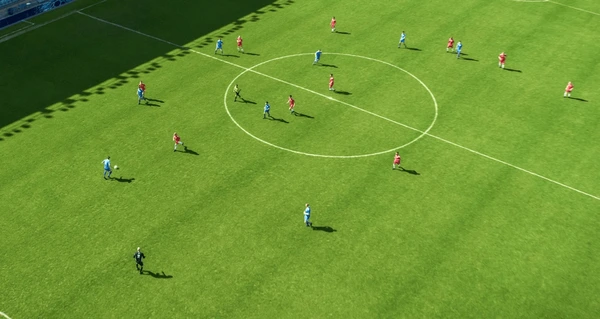
\includegraphics[width=\linewidth]{../data/image_2.png}
    \caption{Original Image}
  \end{subfigure}
  \begin{subfigure}[b]{0.48\linewidth}
    \centering
    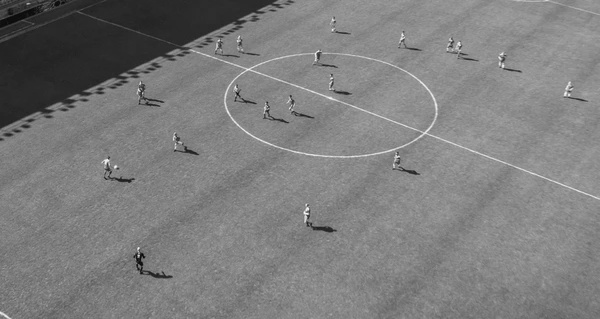
\includegraphics[width=\linewidth]{../edge_detection_steps/01_grayscale.jpg}
    \caption{Grayscale Conversion}
  \end{subfigure}
  \begin{subfigure}[b]{0.48\linewidth}
    \centering
    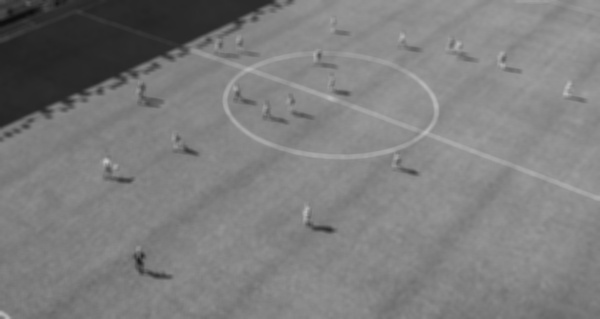
\includegraphics[width=\linewidth]{../edge_detection_steps/02_gaussian_blur.jpg}
    \caption{Gaussian Blur}
  \end{subfigure}
  \begin{subfigure}[b]{0.48\linewidth}
    \centering
    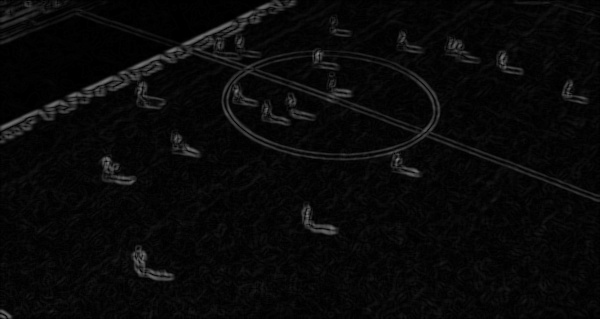
\includegraphics[width=\linewidth]{../edge_detection_steps/03_gradient_magnitude.jpg}
    \caption{Gradient Magnitude}
  \end{subfigure}
  \begin{subfigure}[b]{0.48\linewidth}
    \centering
    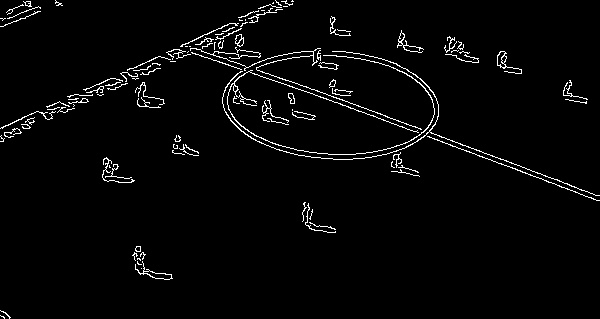
\includegraphics[width=\linewidth]{../edge_detection_steps/04_canny_edges.jpg}
    \caption{Canny Edges}
  \end{subfigure}
  \begin{subfigure}[b]{0.48\linewidth}
    \centering
    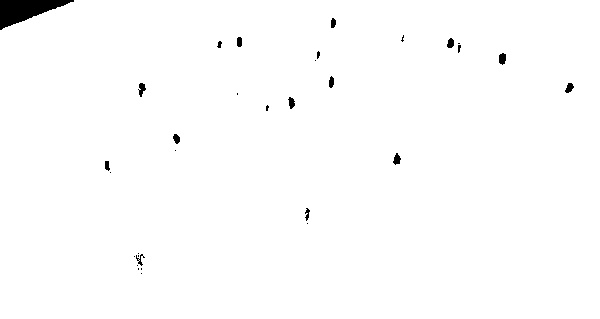
\includegraphics[width=\linewidth]{../edge_detection_steps/05_field_mask.jpg}
    \caption{Field Mask}
  \end{subfigure}
  \begin{subfigure}[b]{0.48\linewidth}
    \centering
    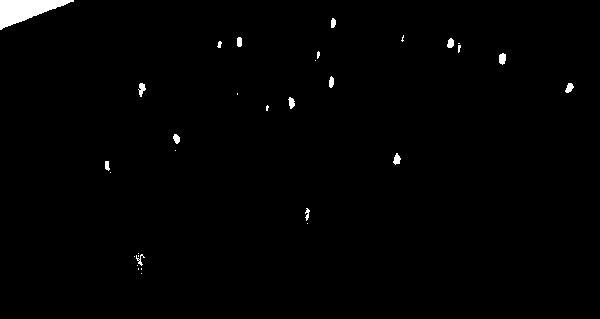
\includegraphics[width=\linewidth]{../edge_detection_steps/06_non_field_mask.jpg}
    \caption{Non-Field Mask}
  \end{subfigure}
  \begin{subfigure}[b]{0.48\linewidth}
    \centering
    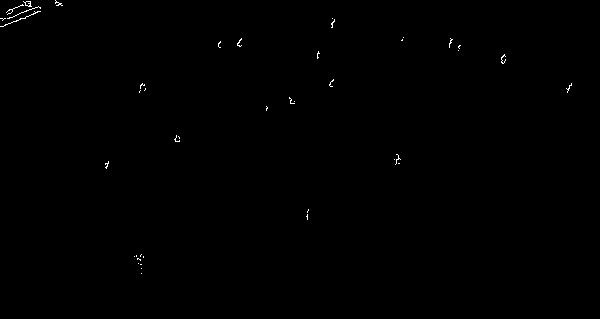
\includegraphics[width=\linewidth]{../edge_detection_steps/07_player_edges.jpg}
    \caption{Player Edges}
  \end{subfigure}
  \begin{subfigure}[b]{0.48\linewidth}
    \centering
    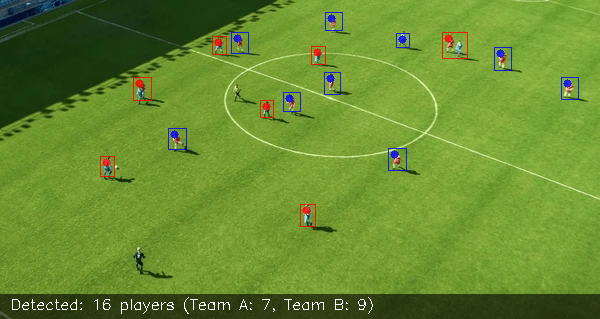
\includegraphics[width=\linewidth]{../edge_detection_steps/09_final_image_2.png}
    \caption{Final Detection}
  \end{subfigure}
  \caption{Step-by-step visualization of the player detection pipeline}
  \label{fig:detection_steps}
\end{figure}

In Figure \ref{fig:detection_results}, we show successful player detection and team classification results on a test image. The system correctly identifies most players on the field and assigns them to the appropriate teams (red and blue bounding boxes).

\begin{figure}[t]
  \centering
  \begin{subfigure}[b]{0.48\linewidth}
    \centering
    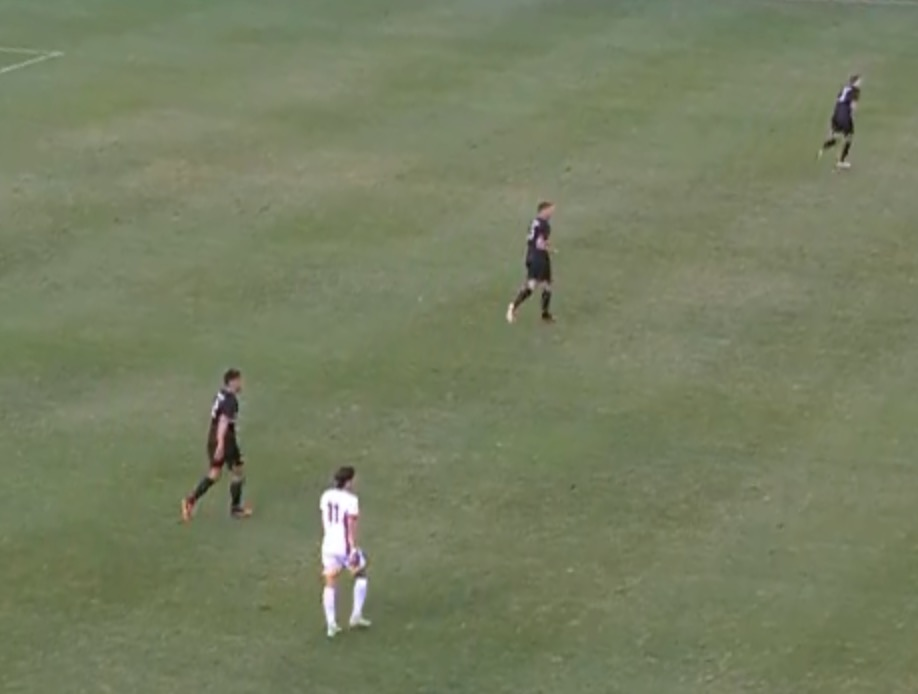
\includegraphics[width=\linewidth]{../data/orginal_image_1.jpeg}
    \caption{Original Image}
  \end{subfigure}
  \begin{subfigure}[b]{0.48\linewidth}
    \centering
    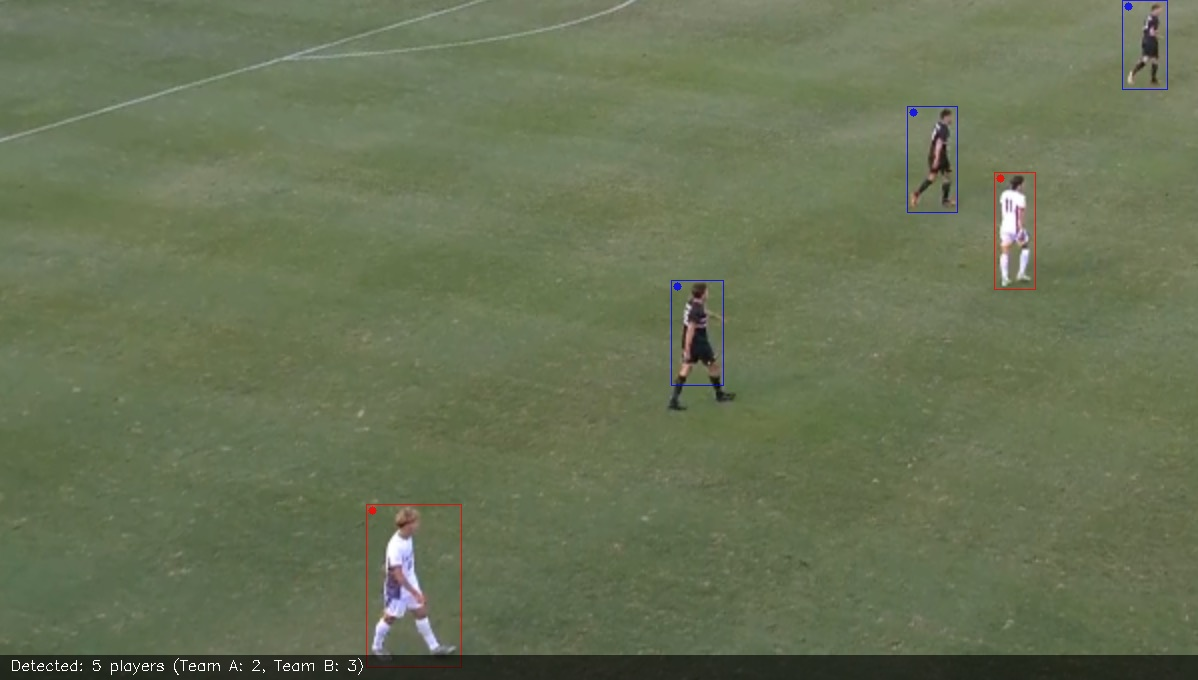
\includegraphics[width=\linewidth]{../edge_detection_steps/results_image_1.jpeg}
    \caption{Detection Results}
  \end{subfigure}
  \caption{Player detection and team classification results}
  \label{fig:detection_results}
\end{figure}

\begin{figure}[t]
  \centering
  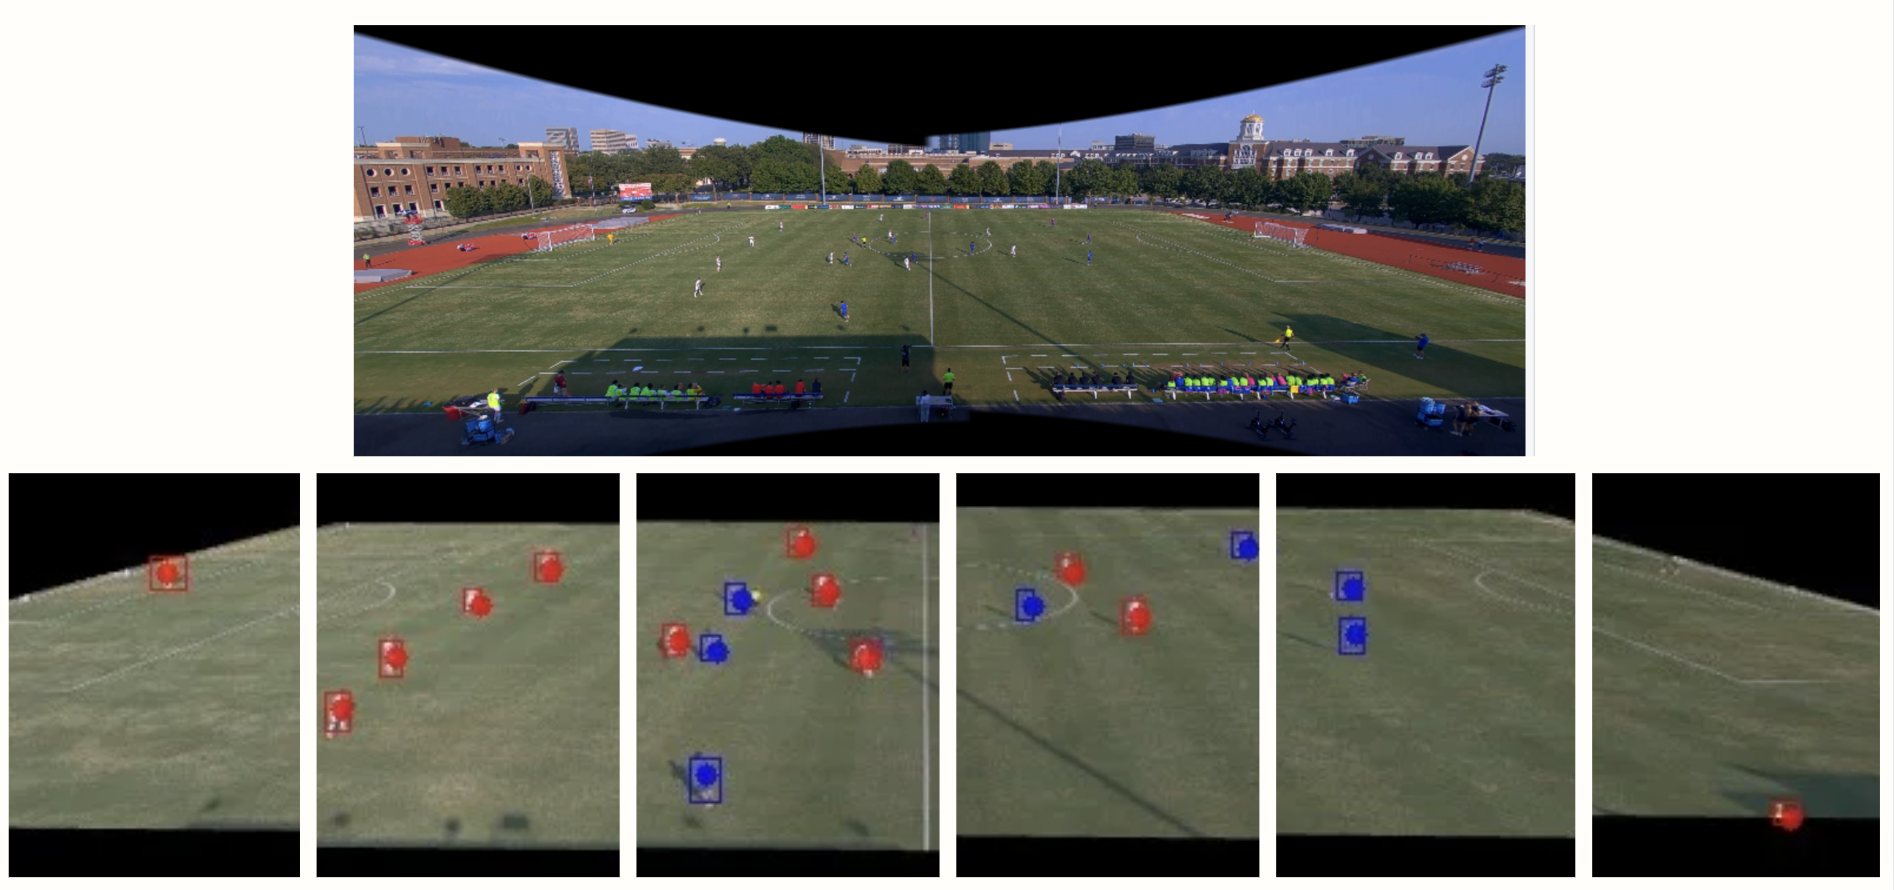
\includegraphics[width=\linewidth]{../edge_detection_steps/results_3.png}
  \caption{Results of player detection and team classification applied to a panoramic image that was split into segments for processing.}
  \label{fig:panoramic_results}
\end{figure}

\subsection{Failure Cases}

Our system is not without limitations. Figure \ref{fig:failure_case} shows a case where the system struggled with complex scenarios:

\begin{figure}[t]
  \centering
  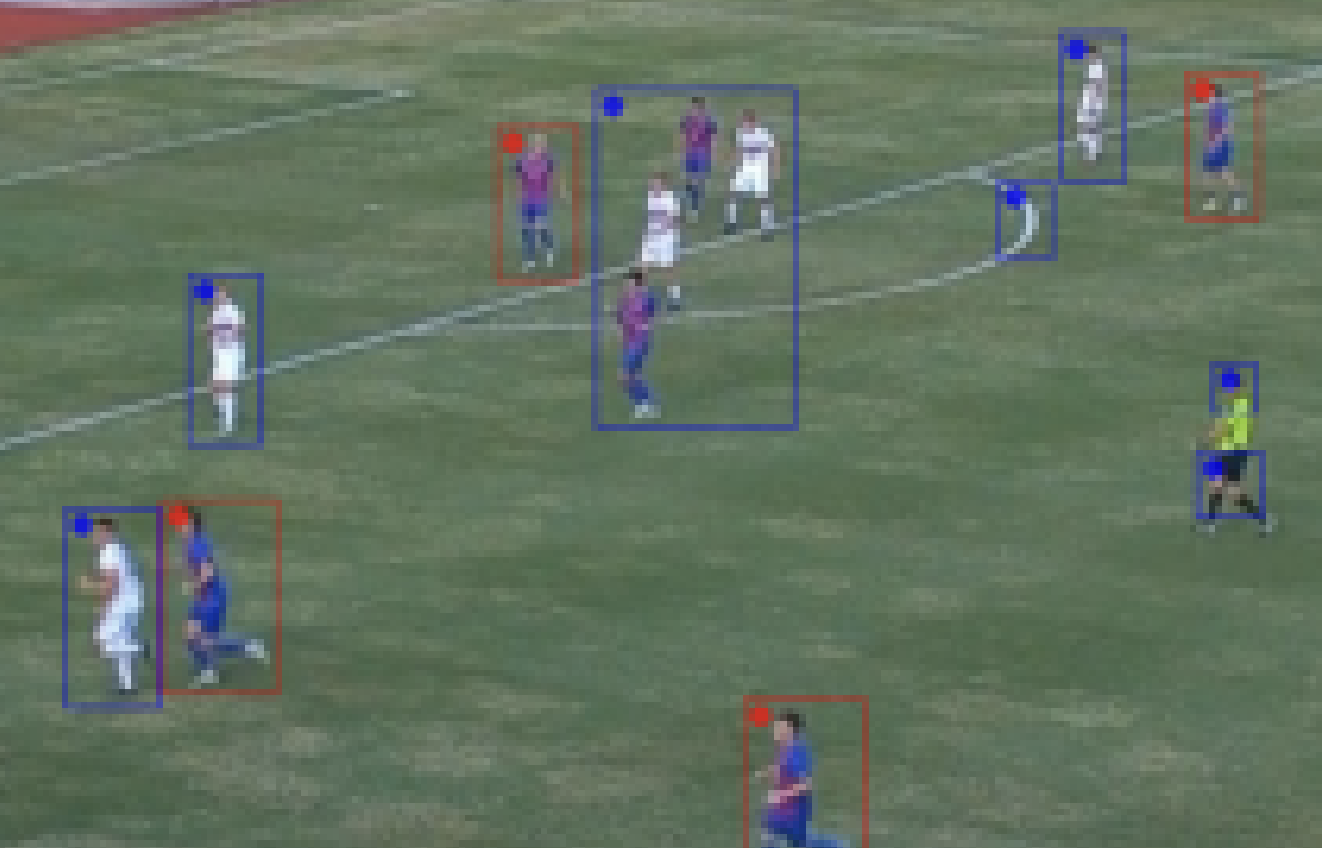
\includegraphics[width=0.9\linewidth]{../edge_detection_steps/results_fail.jpeg}
  \caption{Example of a failure case: The system struggles with tightly grouped players and complex backgrounds.}
  \label{fig:failure_case}
\end{figure}

Common failure modes include:
\begin{itemize}
    \item False positives with field lines and other elements
    \item Merging multiple players into a single detection when they are close together
    \item Classifying the referee as a player
\end{itemize}

\section{Conclusion}
\label{sec:conclusion}

This paper presented SoccerVision, a system for soccer player detection and team classification using classical computer vision techniques. Our approach demonstrates that effective results can be achieved without relying on deep learning or complex machine learning libraries, making it accessible for educational purposes and deployable in environments with limited computational resources.

The key contributions of this work include:
\begin{itemize}
    \item A comprehensive player detection pipeline combining edge detection with field segmentation
    \item A custom binary k-means clustering implementation optimized for team classification
\end{itemize}

\subsection{Future Work}

Several avenues for future improvement exist:
\begin{itemize}
    \item Incorporating temporal information across video frames to improve detection stability
    \item Adding player tracking capabilities to maintain identity across frames. Extending the system to detect additional elements such as the ball, referees, and goalkeepers
\end{itemize}

\section{Individual Contributions}
\label{sec:contributions}

This project was developed by Abel Dagne and Laszlo Bollyky for CS 131. The contributions were split as follows:

\textbf{Abel Dagne:}
\begin{itemize}
    \item Design and implementation of the player detection pipeline
    \item Implementation of the edge detection and field segmentation algorithms
    \item Development of the non-maximum suppression for overlapping detections
    \item Extensive testing and performance optimization of the detection system
    \item Documentation of the player detection methodology
    \item Implementation of the visualization pipeline for intermediate detection steps
\end{itemize}

\textbf{Laszlo Bollyky:}
\begin{itemize}
    \item Design and implementation of the team classification system
    \item Development of the custom k-means clustering algorithm
    \item Implementation of the HSV color feature extraction
    \item Assembly and curation of the test dataset
    \item Creation of the panoramic image preprocessing pipeline
    \item Documentation of the team classification methodology
\end{itemize}


\textbf{AI Tools Used:}
\begin{itemize}
    \item Cursor with Claude 3.7 Sonnet was used as a coding assistant for implementing the pre-processing step to intake the panoramic images and split them into segments for processing. 
    \item We also used Cursor to implement the visualization tools to visualize the intermediate steps of the player detection pipeline.
\end{itemize}

%%%%%%%%% REFERENCES
{\small
\bibliographystyle{ieee_fullname}
\bibliography{egbib}
}

\end{document}
